\begin{frame}{Example}
\begin{overlayarea}{\textwidth}{\textheight}

  \only<1>{
    \vspace{1cm}
    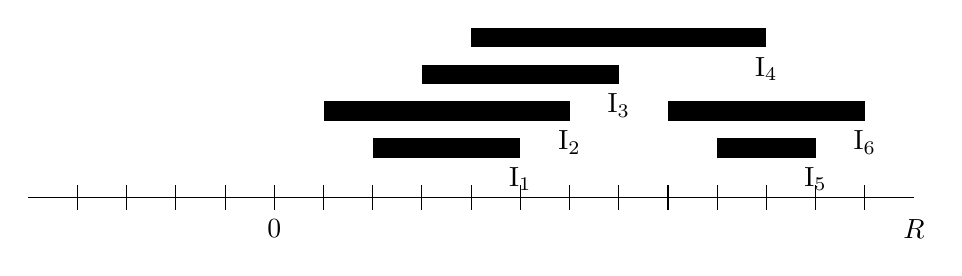
\begin{tikzpicture}[scale=0.625]
      \draw (-5,0) -- (13,0);
      \draw (13,-0.25) node[below]{$\mathbb{R}$};
      \draw (0,-0.25) node[below]{0};
      \foreach \x in {-4,-3,...,12}
        {\draw (\x,-0.25) -- (\x, 0.25);}

      \fill (2,0.80) rectangle (5,1.20);
      \draw (5, 0.80) node[below]{$\mathrm{I_{1}}$};
      \fill (1,1.55) rectangle (6,1.95);
      \draw (6, 1.55) node[below]{$\mathrm{I_{2}}$};
      \fill (3,2.30) rectangle (7,2.70);
      \draw (7, 2.30) node[below]{$\mathrm{I_{3}}$};
      \fill (4,3.05) rectangle (10,3.45);
      \draw (10, 3.05) node[below]{$\mathrm{I_{4}}$};
      \fill (9,0.80) rectangle (11,1.20);
      \draw (11, 0.80) node[below]{$\mathrm{I_{5}}$};
      \fill (8,1.55) rectangle (12,1.95);
      \draw (12, 1.55) node[below]{$\mathrm{I_{6}}$};
    \end{tikzpicture}
  }

  \only<2>{
      \vspace{1cm}
    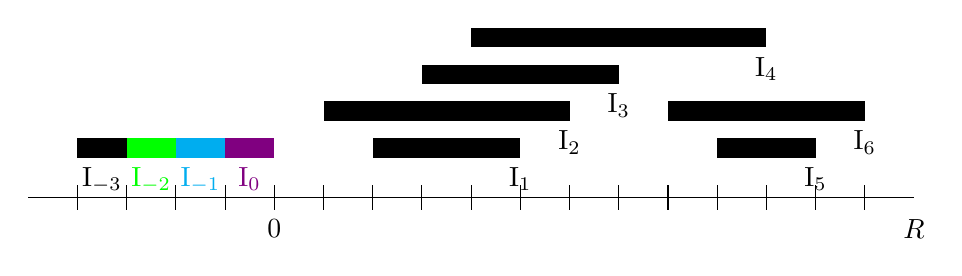
\begin{tikzpicture}[scale=0.625]
      \draw (-5,0) -- (13,0);
      \draw (13,-0.25) node[below]{$\mathbb{R}$};
      \draw (0,-0.25) node[below]{0};
      \foreach \x in {-4,-3,...,12}
        {\draw (\x,-0.25) -- (\x, 0.25);}

      \fill (-4,0.80) rectangle (-3,1.20);
      \draw (-3.5, 0.80) node[below]{$\mathrm{I_{-3}}$};
      \fill[color = green] (-3,0.80) rectangle (-2,1.20);
      \draw (-2.5, 0.80) node[below]{\textcolor{green}{$\mathrm{I_{-2}}$}};
      \fill[color = cyan] (-2,0.80) rectangle (-1,1.20);
      \draw (-1.5, 0.80) node[below]{\textcolor{cyan}{$\mathrm{I_{-1}}$}};
      \fill[color = violet] (-1,0.80) rectangle (0,1.20);
      \draw (-0.5, 0.80) node[below]{\textcolor{violet}{$\mathrm{I_{0}}$}};
      \fill (2,0.80) rectangle (5,1.20);
      \draw (5, 0.80) node[below]{$\mathrm{I_{1}}$};
      \fill (1,1.55) rectangle (6,1.95);
      \draw (6, 1.55) node[below]{$\mathrm{I_{2}}$};
      \fill (3,2.30) rectangle (7,2.70);
      \draw (7, 2.30) node[below]{$\mathrm{I_{3}}$};
      \fill (4,3.05) rectangle (10,3.45);
      \draw (10, 3.05) node[below]{$\mathrm{I_{4}}$};
      \fill (9,0.80) rectangle (11,1.20);
      \draw (11, 0.80) node[below]{$\mathrm{I_{5}}$};
      \fill (8,1.55) rectangle (12,1.95);
      \draw (12, 1.55) node[below]{$\mathrm{I_{6}}$};
    \end{tikzpicture}
    \begin{block}{Sets}
    \{$\mathrm{I_{-3}}$\} \{\textcolor{green}{$\mathrm{I_{-2}}$}\} \{\textcolor{cyan}{$\mathrm{I_{-1}}$}\} \{\textcolor{violet}{$\mathrm{I_{0}}$}\} \{$\mathrm{I_{1}}$\} \{$\mathrm{I_{2}}$\} \{$\mathrm{I_{3}}$\} \{$\mathrm{I_{4}}$\} \{$\mathrm{I_{5}}$\} \{$\mathrm{I_{6}}$\}
    \end{block}
  }

  \only<3>{
      \vspace{1cm}
    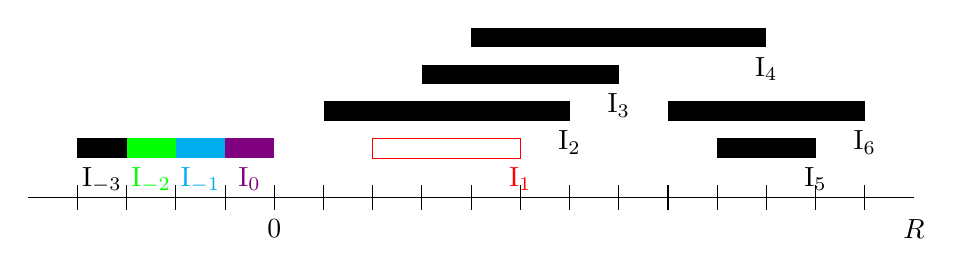
\begin{tikzpicture}[scale=0.625]
      \draw (-5,0) -- (13,0);
      \draw (13,-0.25) node[below]{$\mathbb{R}$};
      \draw (0,-0.25) node[below]{0};
      \foreach \x in {-4,-3,...,12}
        {\draw (\x,-0.25) -- (\x, 0.25);}

      \fill (-4,0.80) rectangle (-3,1.20);
      \draw (-3.5, 0.80) node[below]{$\mathrm{I_{-3}}$};
      \fill[color = green] (-3,0.80) rectangle (-2,1.20);
      \draw (-2.5, 0.80) node[below]{\textcolor{green}{$\mathrm{I_{-2}}$}};
      \fill[color = cyan] (-2,0.80) rectangle (-1,1.20);
      \draw (-1.5, 0.80) node[below]{\textcolor{cyan}{$\mathrm{I_{-1}}$}};
      \fill[color = violet] (-1,0.80) rectangle (0,1.20);
      \draw (-0.5, 0.80) node[below]{\textcolor{violet}{$\mathrm{I_{0}}$}};
      \draw [color = red] (2,0.80) rectangle (5,1.20);
      \draw (5, 0.80) node[below]{\textcolor{red}{$\mathrm{I_{1}}$}};
      \fill (1,1.55) rectangle (6,1.95);
      \draw (6, 1.55) node[below]{$\mathrm{I_{2}}$};
      \fill (3,2.30) rectangle (7,2.70);
      \draw (7, 2.30) node[below]{$\mathrm{I_{3}}$};
      \fill (4,3.05) rectangle (10,3.45);
      \draw (10, 3.05) node[below]{$\mathrm{I_{4}}$};
      \fill (9,0.80) rectangle (11,1.20);
      \draw (11, 0.80) node[below]{$\mathrm{I_{5}}$};
      \fill (8,1.55) rectangle (12,1.95);
      \draw (12, 1.55) node[below]{$\mathrm{I_{6}}$};
    \end{tikzpicture}
    \begin{block}{Sets}
    \{$\mathrm{I_{-3}}$\} \{\textcolor{green}{$\mathrm{I_{-2}}$}\} \{\textcolor{cyan}{$\mathrm{I_{-1}}$}\} \{\textcolor{violet}{$\mathrm{I_{0}}$}\} \{$\mathrm{I_{1}}$\} \{$\mathrm{I_{2}}$\} \{$\mathrm{I_{3}}$\} \{$\mathrm{I_{4}}$\} \{$\mathrm{I_{5}}$\} \{$\mathrm{I_{6}}$\}
    \end{block}
    \begin{block}{Operations}
      \begin{columns}[T]
      \begin{column}{.48\textwidth}
        \begin{itemize}
          \item[$\bullet$]i = 1
          \item[$\bullet$]adjacent($\mathrm{I_{i}}$) = $\mathrm{I_{0}}$
          \item[$\bullet$]Best fit leader = find(adjacent($\mathrm{I_{i}}$)) = $\mathrm{I_{0}}$
        \end{itemize}
      \end{column}
      \begin{column}{.48\textwidth}
        \begin{itemize}
          \item[\textcolor{red}{$\bullet$}]\textcolor{red}{color($\mathrm{I_{i}}$)$\leftarrow$color($\mathrm{I_{j}}$)}
          \item[$\bullet$]find($\mathrm{I_{j-1}}$) = $\mathrm{I_{-1}}$
          \item[\textcolor{red}{$\bullet$}]\textcolor{red}{union($\mathrm{I_{j}}$,find($\mathrm{I_{j-1}}$))}
        \end{itemize}
      \end{column}
      \end{columns}  
    \end{block}
  }
    \only<4>{
    \vspace{1cm}
    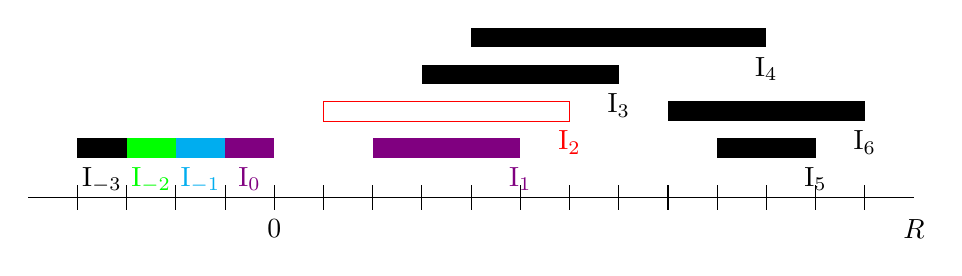
\begin{tikzpicture}[scale=0.625]
      \draw (-5,0) -- (13,0);
      \draw (13,-0.25) node[below]{$\mathbb{R}$};
      \draw (0,-0.25) node[below]{0};
      \foreach \x in {-4,-3,...,12}
        {\draw (\x,-0.25) -- (\x, 0.25);}

      \fill (-4,0.80) rectangle (-3,1.20);
      \draw (-3.5, 0.80) node[below]{$\mathrm{I_{-3}}$};
      \fill[color=green] (-3,0.80) rectangle (-2,1.20);
      \draw (-2.5, 0.80) node[below]{\textcolor{green}{$\mathrm{I_{-2}}$}};
      \fill[color=cyan] (-2,0.80) rectangle (-1,1.20);
      \draw (-1.5, 0.80) node[below]{\textcolor{cyan}{$\mathrm{I_{-1}}$}};
      \fill[color=violet] (-1,0.80) rectangle (0,1.20);
      \draw (-0.5, 0.80) node[below]{\textcolor{violet}{$\mathrm{I_{0}}$}};
      \fill[color=violet] (2,0.80) rectangle (5,1.20);
      \draw (5, 0.80) node[below]{\textcolor{violet}{$\mathrm{I_{1}}$}};
      \draw[color=red] (1,1.55) rectangle (6,1.95);
      \draw (6, 1.55) node[below]{\textcolor{red}{$\mathrm{I_{2}}$}};
      \fill (3,2.30) rectangle (7,2.70);
      \draw (7, 2.30) node[below]{$\mathrm{I_{3}}$};
      \fill (4,3.05) rectangle (10,3.45);
      \draw (10, 3.05) node[below]{$\mathrm{I_{4}}$};
      \fill (9,0.80) rectangle (11,1.20);
      \draw (11, 0.80) node[below]{$\mathrm{I_{5}}$};
      \fill (8,1.55) rectangle (12,1.95);
      \draw (12, 1.55) node[below]{$\mathrm{I_{6}}$};
    \end{tikzpicture}
    \begin{block}{Sets}
    \{$\mathrm{I_{-3}}$\} \{\textcolor{green}{$\mathrm{I_{-2}}$}\} \{\textcolor{cyan}{$\mathrm{I_{-1}}$},\textcolor{violet}{$\mathrm{I_{0}}$}\} \{\textcolor{violet}{$\mathrm{I_{1}}$}\} \{$\mathrm{I_{2}}$\} \{$\mathrm{I_{3}}$\} \{$\mathrm{I_{4}}$\} \{$\mathrm{I_{5}}$\} \{$\mathrm{I_{6}}$\}
    \end{block}
    \begin{block}{Operations}
      \begin{columns}[T]
      \begin{column}{.48\textwidth}
        \begin{itemize}
          \item[$\bullet$]i = 2
          \item[$\bullet$]adjacent($\mathrm{I_{2}}$) = $\mathrm{I_{0}}$
          \item[$\bullet$]find($\mathrm{I_{0}}$) = $\mathrm{I_{-1}}$
        \end{itemize}
      \end{column}
      \begin{column}{.48\textwidth}
        \begin{itemize}
          \item[\textcolor{red}{$\bullet$}]\textcolor{red}{color($\mathrm{I_{2}}$)$\leftarrow$color($\mathrm{I_{-1}}$)}
          \item[$\bullet$]find($\mathrm{I_{-2}}$) = $\mathrm{I_{-2}}$
          \item[\textcolor{red}{$\bullet$}]\textcolor{red}{union($\mathrm{I_{-1}},\mathrm{I_{-2}}$)}
        \end{itemize}
      \end{column}
      \end{columns}  
    \end{block}
  }
  
  \only<5>{
    \vspace{1cm}
    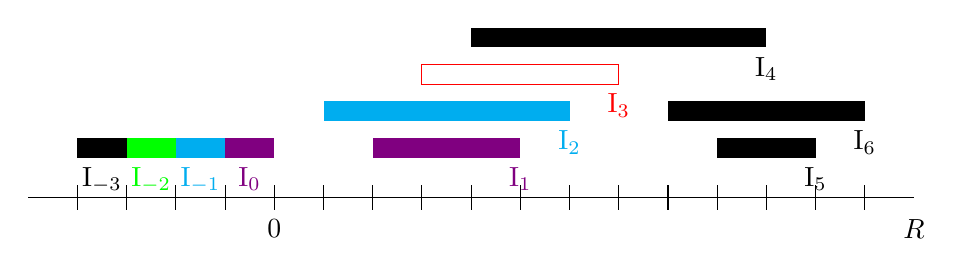
\begin{tikzpicture}[scale=0.625]
      \draw (-5,0) -- (13,0);
      \draw (13,-0.25) node[below]{$\mathbb{R}$};
      \draw (0,-0.25) node[below]{0};
      \foreach \x in {-4,-3,...,12}
        {\draw (\x,-0.25) -- (\x, 0.25);}

      \fill (-4,0.80) rectangle (-3,1.20);
      \draw (-3.5, 0.80) node[below]{$\mathrm{I_{-3}}$};
      \fill[color=green] (-3,0.80) rectangle (-2,1.20);
      \draw (-2.5, 0.80) node[below]{\textcolor{green}{$\mathrm{I_{-2}}$}};
      \fill[color=cyan] (-2,0.80) rectangle (-1,1.20);
      \draw (-1.5, 0.80) node[below]{\textcolor{cyan}{$\mathrm{I_{-1}}$}};
      \fill[color=violet] (-1,0.80) rectangle (0,1.20);
      \draw (-0.5, 0.80) node[below]{\textcolor{violet}{$\mathrm{I_{0}}$}};
      \fill[color=violet] (2,0.80) rectangle (5,1.20);
      \draw (5, 0.80) node[below]{\textcolor{violet}{$\mathrm{I_{1}}$}};
      \fill[color=cyan] (1,1.55) rectangle (6,1.95);
      \draw (6, 1.55) node[below]{\textcolor{cyan}{$\mathrm{I_{2}}$}};
      \draw[color=red] (3,2.30) rectangle (7,2.70);
      \draw (7, 2.30) node[below]{\textcolor{red}{$\mathrm{I_{3}}$}};
      \fill (4,3.05) rectangle (10,3.45);
      \draw (10, 3.05) node[below]{$\mathrm{I_{4}}$};
      \fill (9,0.80) rectangle (11,1.20);
      \draw (11, 0.80) node[below]{$\mathrm{I_{5}}$};
      \fill (8,1.55) rectangle (12,1.95);
      \draw (12, 1.55) node[below]{$\mathrm{I_{6}}$};
    \end{tikzpicture}
    \begin{block}{Sets}
    \{$\mathrm{I_{-3}}$\} \{\textcolor{green}{$\mathrm{I_{-2}}$},\textcolor{cyan}{$\mathrm{I_{-1}}$},\textcolor{violet}{$\mathrm{I_{0}}$}\} \{\textcolor{violet}{$\mathrm{I_{1}}$}\} \{\textcolor{cyan}{$\mathrm{I_{2}}$}\} \{$\mathrm{I_{3}}$\} \{$\mathrm{I_{4}}$\} \{$\mathrm{I_{5}}$\} \{$\mathrm{I_{6}}$\}
    \end{block}
    \begin{block}{Operations}
      \begin{columns}[T]
      \begin{column}{.48\textwidth}
        \begin{itemize}
          \item[$\bullet$]i = 3
          \item[$\bullet$]adjacent($\mathrm{I_{3}}$) = $\mathrm{I_{0}}$
          \item[$\bullet$]find($\mathrm{I_{0}}$) = $\mathrm{I_{-2}}$
        \end{itemize}
      \end{column}
      \begin{column}{.48\textwidth}
        \begin{itemize}
          \item[\textcolor{red}{$\bullet$}]\textcolor{red}{color($\mathrm{I_{3}}$)$\leftarrow$color($\mathrm{I_{-2}}$)}
          \item[$\bullet$]find($\mathrm{I_{-3}}$) = $\mathrm{I_{-3}}$
          \item[\textcolor{red}{$\bullet$}]\textcolor{red}{union($\mathrm{I_{-2}},\mathrm{I_{-3}}$)}
        \end{itemize}
      \end{column}
      \end{columns}  
    \end{block}
  }
  
  
    \only<6>{
    \vspace{1cm}
    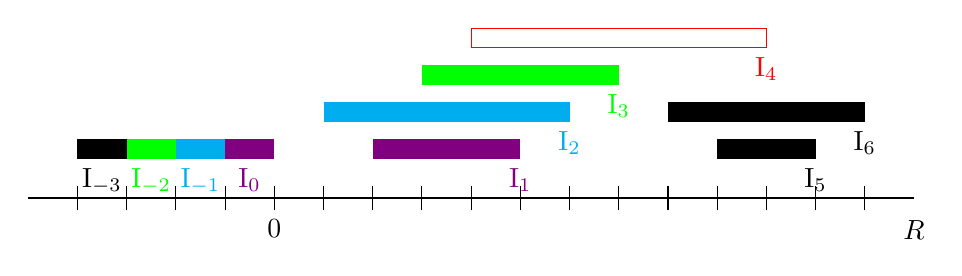
\begin{tikzpicture}[scale=0.625]
      \draw (-5,0) -- (13,0);
      \draw (13,-0.25) node[below]{$\mathbb{R}$};
      \draw (0,-0.25) node[below]{0};
      \foreach \x in {-4,-3,...,12}
        {\draw (\x,-0.25) -- (\x, 0.25);}

      \fill (-4,0.80) rectangle (-3,1.20);
      \draw (-3.5, 0.80) node[below]{$\mathrm{I_{-3}}$};
      \fill[color=green] (-3,0.80) rectangle (-2,1.20);
      \draw (-2.5, 0.80) node[below]{\textcolor{green}{$\mathrm{I_{-2}}$}};
      \fill[color=cyan] (-2,0.80) rectangle (-1,1.20);
      \draw (-1.5, 0.80) node[below]{\textcolor{cyan}{$\mathrm{I_{-1}}$}};
      \fill[color=violet] (-1,0.80) rectangle (0,1.20);
      \draw (-0.5, 0.80) node[below]{\textcolor{violet}{$\mathrm{I_{0}}$}};
      \fill[color=violet] (2,0.80) rectangle (5,1.20);
      \draw (5, 0.80) node[below]{\textcolor{violet}{$\mathrm{I_{1}}$}};
      \fill[color=cyan] (1,1.55) rectangle (6,1.95);
      \draw (6, 1.55) node[below]{\textcolor{cyan}{$\mathrm{I_{2}}$}};
      \fill[color=green] (3,2.30) rectangle (7,2.70);
      \draw (7, 2.30) node[below]{\textcolor{green}{$\mathrm{I_{3}}$}};
      \draw[color=red] (4,3.05) rectangle (10,3.45);
      \draw (10, 3.05) node[below]{\textcolor{red}{$\mathrm{I_{4}}$}};
      \fill (9,0.80) rectangle (11,1.20);
      \draw (11, 0.80) node[below]{$\mathrm{I_{5}}$};
      \fill (8,1.55) rectangle (12,1.95);
      \draw (12, 1.55) node[below]{$\mathrm{I_{6}}$};
    \end{tikzpicture}
    \begin{block}{Sets}
    \{$\mathrm{I_{-3}}$,\textcolor{green}{$\mathrm{I_{-2}}$},\textcolor{cyan}{$\mathrm{I_{-1}}$},\textcolor{violet}{$\mathrm{I_{0}}$}\} \{\textcolor{violet}{$\mathrm{I_{1}}$}\} \{\textcolor{cyan}{$\mathrm{I_{2}}$}\} \{\textcolor{green}{$\mathrm{I_{3}}$}\} \{$\mathrm{I_{4}}$\} \{$\mathrm{I_{5}}$\} \{$\mathrm{I_{6}}$\}
    \end{block}
    \begin{block}{Operations}
      \begin{columns}[T]
      \begin{column}{.48\textwidth}
        \begin{itemize}
          \item[$\bullet$]i = 4
          \item[$\bullet$]adjacent($\mathrm{I_{4}}$) = $\mathrm{I_{0}}$
          \item[$\bullet$]find($\mathrm{I_{0}}$) = $\mathrm{I_{-3}}$
        \end{itemize}
      \end{column}
      \begin{column}{.48\textwidth}
        \begin{itemize}
          \item[\textcolor{red}{$\bullet$}]\textcolor{red}{color($\mathrm{I_{4}}$)$\leftarrow$0}
          \item[$\bullet$]find($\mathrm{I_{i-1}}$) = $\mathrm{I_{3}}$
          \item[\textcolor{red}{$\bullet$}]\textcolor{red}{union($\mathrm{I_{i}}$,find($\mathrm{I_{i-1}}$))}
        \end{itemize}
      \end{column}
      \end{columns}  
    \end{block}
  }
  
      \only<7>{
    \vspace{1cm}
    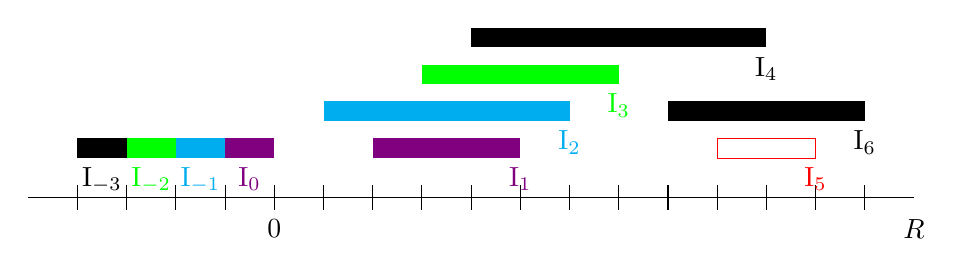
\begin{tikzpicture}[scale=0.625]
      \draw (-5,0) -- (13,0);
      \draw (13,-0.25) node[below]{$\mathbb{R}$};
      \draw (0,-0.25) node[below]{0};
      \foreach \x in {-4,-3,...,12}
        {\draw (\x,-0.25) -- (\x, 0.25);}

      \fill (-4,0.80) rectangle (-3,1.20);
      \draw (-3.5, 0.80) node[below]{$\mathrm{I_{-3}}$};
      \fill[color=green] (-3,0.80) rectangle (-2,1.20);
      \draw (-2.5, 0.80) node[below]{\textcolor{green}{$\mathrm{I_{-2}}$}};
      \fill[color=cyan] (-2,0.80) rectangle (-1,1.20);
      \draw (-1.5, 0.80) node[below]{\textcolor{cyan}{$\mathrm{I_{-1}}$}};
      \fill[color=violet] (-1,0.80) rectangle (0,1.20);
      \draw (-0.5, 0.80) node[below]{\textcolor{violet}{$\mathrm{I_{0}}$}};
      \fill[color=violet] (2,0.80) rectangle (5,1.20);
      \draw (5, 0.80) node[below]{\textcolor{violet}{$\mathrm{I_{1}}$}};
      \fill[color=cyan] (1,1.55) rectangle (6,1.95);
      \draw (6, 1.55) node[below]{\textcolor{cyan}{$\mathrm{I_{2}}$}};
      \fill[color=green] (3,2.30) rectangle (7,2.70);
      \draw (7, 2.30) node[below]{\textcolor{green}{$\mathrm{I_{3}}$}};
      \fill (4,3.05) rectangle (10,3.45);
      \draw (10, 3.05) node[below]{$\mathrm{I_{4}}$};
      \draw[color=red] (9,0.80) rectangle (11,1.20);
      \draw (11, 0.80) node[below]{\textcolor{red}{$\mathrm{I_{5}}$}};
      \fill (8,1.55) rectangle (12,1.95);
      \draw (12, 1.55) node[below]{$\mathrm{I_{6}}$};
    \end{tikzpicture}
    \begin{block}{Sets}
    \{$\mathrm{I_{-3}}$,\textcolor{green}{$\mathrm{I_{-2}}$},\textcolor{cyan}{$\mathrm{I_{-1}}$},\textcolor{violet}{$\mathrm{I_{0}}$}\} \{\textcolor{violet}{$\mathrm{I_{1}}$}\} \{\textcolor{cyan}{$\mathrm{I_{2}}$}\} \{\textcolor{green}{$\mathrm{I_{3}}$},$\mathrm{I_{4}}$\} \{$\mathrm{I_{5}}$\} \{$\mathrm{I_{6}}$\}
    \end{block}
    \begin{block}{Operations}
      \begin{columns}[T]
      \begin{column}{.48\textwidth}
        \begin{itemize}
          \item[$\bullet$]i = 5
          \item[$\bullet$]adjacent($\mathrm{I_{5}}$) = $\mathrm{I_{3}}$
          \item[$\bullet$]find($\mathrm{I_{3}}$) = $\mathrm{I_{3}}$
        \end{itemize}
      \end{column}
      \begin{column}{.48\textwidth}
        \begin{itemize}
          \item[\textcolor{red}{$\bullet$}]\textcolor{red}{color($\mathrm{I_{5}}$)$\leftarrow$color($\mathrm{I_{3}}$)}
          \item[$\bullet$]find($\mathrm{I_{2}}$) = $\mathrm{I_{2}}$
          \item[\textcolor{red}{$\bullet$}]\textcolor{red}{union($\mathrm{I_{3}}$,find($\mathrm{I_{2}}$))}
        \end{itemize}
      \end{column}
      \end{columns}  
    \end{block}
  }
  
   
   \only<8>{
    \vspace{1cm}
    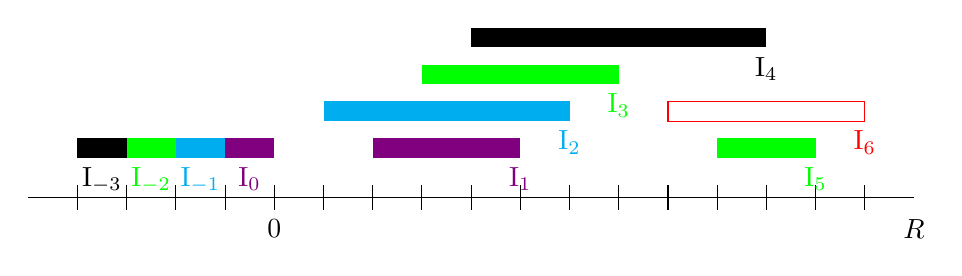
\begin{tikzpicture}[scale=0.625]
      \draw (-5,0) -- (13,0);
      \draw (13,-0.25) node[below]{$\mathbb{R}$};
      \draw (0,-0.25) node[below]{0};
      \foreach \x in {-4,-3,...,12}
        {\draw (\x,-0.25) -- (\x, 0.25);}

      \fill (-4,0.80) rectangle (-3,1.20);
      \draw (-3.5, 0.80) node[below]{$\mathrm{I_{-3}}$};
      \fill[color=green] (-3,0.80) rectangle (-2,1.20);
      \draw (-2.5, 0.80) node[below]{\textcolor{green}{$\mathrm{I_{-2}}$}};
      \fill[color=cyan] (-2,0.80) rectangle (-1,1.20);
      \draw (-1.5, 0.80) node[below]{\textcolor{cyan}{$\mathrm{I_{-1}}$}};
      \fill[color=violet] (-1,0.80) rectangle (0,1.20);
      \draw (-0.5, 0.80) node[below]{\textcolor{violet}{$\mathrm{I_{0}}$}};
      \fill[color=violet] (2,0.80) rectangle (5,1.20);
      \draw (5, 0.80) node[below]{\textcolor{violet}{$\mathrm{I_{1}}$}};
      \fill[color=cyan] (1,1.55) rectangle (6,1.95);
      \draw (6, 1.55) node[below]{\textcolor{cyan}{$\mathrm{I_{2}}$}};
      \fill[color=green] (3,2.30) rectangle (7,2.70);
      \draw (7, 2.30) node[below]{\textcolor{green}{$\mathrm{I_{3}}$}};
      \fill (4,3.05) rectangle (10,3.45);
      \draw (10, 3.05) node[below]{$\mathrm{I_{4}}$};
      \fill[color=green] (9,0.80) rectangle (11,1.20);
      \draw (11, 0.80) node[below]{\textcolor{green}{$\mathrm{I_{5}}$}};
      \draw[color=red] (8,1.55) rectangle (12,1.95);
      \draw (12, 1.55) node[below]{\textcolor{red}{$\mathrm{I_{6}}$}};
    \end{tikzpicture}
    \begin{block}{Sets}
    \{$\mathrm{I_{-3}}$,\textcolor{green}{$\mathrm{I_{-2}}$},\textcolor{cyan}{$\mathrm{I_{-1}}$},\textcolor{violet}{$\mathrm{I_{0}}$}\} \{\textcolor{violet}{$\mathrm{I_{1}}$}\} \{\textcolor{cyan}{$\mathrm{I_{2}}$},\textcolor{green}{$\mathrm{I_{3}}$},$\mathrm{I_{4}}$\} \{\textcolor{green}{$\mathrm{I_{5}}$}\} \{$\mathrm{I_{6}}$\}
    \end{block}
    \begin{block}{Operations}
      \begin{columns}[T]
      \begin{column}{.48\textwidth}
        \begin{itemize}
          \item[$\bullet$]i = 6
          \item[$\bullet$]adjacent($\mathrm{I_{6}}$) = $\mathrm{I_{3}}$
          \item[$\bullet$]find($\mathrm{I_{3}}$) = $\mathrm{I_{2}}$
        \end{itemize}
      \end{column}
      \begin{column}{.48\textwidth}
        \begin{itemize}
          \item[\textcolor{red}{$\bullet$}]\textcolor{red}{color($\mathrm{I_{6}}$)$\leftarrow$color($\mathrm{I_{2}}$)}
          \item[$\bullet$]find($\mathrm{I_{1}}$) = $\mathrm{I_{1}}$
          \item[\textcolor{red}{$\bullet$}]\textcolor{red}{union($\mathrm{I_{2}}$,find($\mathrm{I_{1}}$))}
        \end{itemize}
      \end{column}
      \end{columns}  
    \end{block}
  }
  
  
     \only<9>{
    \vspace{1cm}
    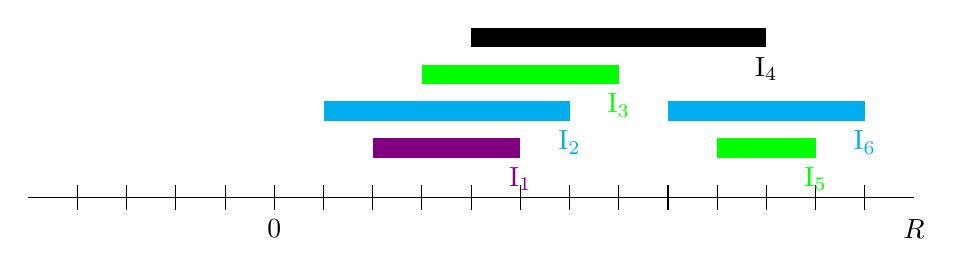
\begin{tikzpicture}[scale=0.625]
      \draw (-5,0) -- (13,0);
      \draw (13,-0.25) node[below]{$\mathbb{R}$};
      \draw (0,-0.25) node[below]{0};
      \foreach \x in {-4,-3,...,12}
        {\draw (\x,-0.25) -- (\x, 0.25);}

      \fill[color=violet] (2,0.80) rectangle (5,1.20);
      \draw (5, 0.80) node[below]{\textcolor{violet}{$\mathrm{I_{1}}$}};
      \fill[color=cyan] (1,1.55) rectangle (6,1.95);
      \draw (6, 1.55) node[below]{\textcolor{cyan}{$\mathrm{I_{2}}$}};
      \fill[color=green] (3,2.30) rectangle (7,2.70);
      \draw (7, 2.30) node[below]{\textcolor{green}{$\mathrm{I_{3}}$}};
      \fill (4,3.05) rectangle (10,3.45);
      \draw (10, 3.05) node[below]{$\mathrm{I_{4}}$};
      \fill[color=green] (9,0.80) rectangle (11,1.20);
      \draw (11, 0.80) node[below]{\textcolor{green}{$\mathrm{I_{5}}$}};
      \fill[color=cyan] (8,1.55) rectangle (12,1.95);
      \draw (12, 1.55) node[below]{\textcolor{cyan}{$\mathrm{I_{6}}$}};
    \end{tikzpicture}
    \begin{block}{Sets}
    \{$\mathrm{I_{-3}}$,\textcolor{green}{$\mathrm{I_{-2}}$},\textcolor{cyan}{$\mathrm{I_{-1}}$},\textcolor{violet}{$\mathrm{I_{0}}$}\} \{\textcolor{violet}{$\mathrm{I_{1}}$},\textcolor{cyan}{$\mathrm{I_{2}}$},\textcolor{green}{$\mathrm{I_{3}}$},$\mathrm{I_{4}}$\} \{\textcolor{green}{$\mathrm{I_{5}}$}\} \{\textcolor{cyan}{$\mathrm{I_{6}}$}\}
    \end{block}
  }
  
\end{overlayarea}
\end{frame}